\chapter{Method}
Given the aim of this project, we now present the methodology. We then present the three cases that are of attention in this project.


\section{Research Methodology}
The aim of this project is to develop a method of analysis that identifies hidden relations in a document database. To perform this, an inductive research design has been taken. Starting off by studying a few specific cases, the expectation is to find some pattern leading to a broader generalization. From there, tentative hypothesis will be formulated which later will be tested and hopefully conveyed into a final conclusion.

\section{Research Design}
% To identify relevant cases, interviews will be held
Taking the inductive approach, the first thing to do is to identify important and representative cases. Thus, the research starts with interviewing analysts at Recorded Future with the result being a list of questions related to their data that are hard to answer based on the existing database and software. This will give us information about what kind of relations that are interesting to look at from a security analyst perspective.

\section{Validation} 
The final step of the study concerns validation. The developed method must be validated to tell whether it is performing well or not. The validation will be performed on a sample of chosen cases, for which the answer is known. The answer could be figured out by for instance perform extensive analysis in multiple steps with the existing database and software.

\section{Introduction to the Data Set \label{dataset}}
The data of Recorded Future is comprised of entities, e.g. a country, a person or a company. They are in turn often a component in an ontology, such as Stockholm being part of Sweden. Another central concept is references, often connecting two entities. References are a report or text fragment related to a specific event. Furthermore, there is metadata that can be different sorts of data related to entities and events, such as a time interval or type of entity or event.

The data is fetched by queries using Recorded Future's API. The output is a file in JSON format. As previously mentioned, the database contains a lot of information. Thus, it is essential that only a subset of the data is fetched. This leads to the issue of querying the right information and only the right information. To be able to answer a question, we want to have all the necessary information at hand without dealing with too much information. This is based on two reasons; querying information takes time and the more data the more complexity arises.

One difficulty with the data is that some parts are implicit. Since Recorded Future are dealing with natural language processing there are cases when all the information about an event is not available. For instance, if someone on the Internet is writing about a cyber attack they might mention an attacker and malware without specifying the target, hence creating implicit data. 

Another important aspect is that the data does not reflect the real world but what users on Internet find interesting to report. Hence, on one hand there might be some information missing, while there on the other hand may be much data on one single event due to various reasons. An example of the latter case is if Donald Trump's personal computer would be hacked by a hacker representing Anonymous. Due to the popularity of both Trump and Anonymous, it is likely that many people writes about this all over the Internet resulting in many references about this specific happening. Thus, the question arises whether there have been multiple attacks or only one. Studying the time of the reports may reveal a lot of information enabling to answer the previous question however there might be cases where there is periodic interest to report about a certain happening. The latter is far more ambiguous.

\section{Extracting Relations From a Document Database}
% Motivate the need to use a graph database
To reduce the time spent on extracting the right kind of data, a graph database has been created

% Introduction to Neo4j
Neo4j is a graph database management system that has a query language Cypher and let the user interact with 

% How is the extraction and import to Neo4j performed?
In many cases, document databases has a nested structure. Thus, it is necessary to flatten out the data

\section{Graph Representation}
Data modeling with graphs are highly domain dependent and highly dependent on what type of question one is trying to answer. Thus, according to \citet{robinson2013}, the following approach should be taken:
\begin{itemize}
    \item Describe the goals that motivate the model.
    \item Rewrite the goals as questions to ask the domain.
    \item Identify the entities and the relationships that appear in these questions. 
    \item Translate the entities and relationships into Cypher path expressions.
    \item Express the questions we want to ask of our domain as graph patterns using path expressions similar to the ones we used to model the domain. 
\end{itemize}

\section{Revealing Hidden Relations}

% Motivate the choice of algorithms
The usefulness of the algorithms and measures highly depends on the task \cite{fouss2016algorithms}. It is therefore necessary to perform empirical tests and validate the relevance. 

Algorithms for analysis has been chosen to be as simple as possible yet give a satisfactory result. 


\section{Introduction to the cases}
Below we present the four cases which has been studied. They were chosen to give a representative view of the questions one might want to address using a graph representation. Also, the cases have been chosen to show the width of uses that a graph representation could cover.

\subsection{Gh0st RAT Controllers}
Gh0st RAT (Remote Access Terminal) is a trojan horse used to hack and take control of computers in real-time. The malware has been used to hack some of the most sensitive computers in the world.

Our data consists of NetFlow data related to a number of IP addresses that have been identified as Ghost RAT controllers. The data is annotated such that known RAT controllers have been annotated with the label \textit{Ghost}. There is also information of the IP traffic such that it is known which IP address that has communicated with whom. Thus, in this case our graph model consists of IP addresses as nodes and a relation ``COMMUNICATED'' between them if they have communicated. The graph is modelled as an undirected graph, since the RAT controller-slave communication can be initiated in any direction.

We have two similar data sets. The first set is based on 21831 NetFlow records collected during the first months of 2017. In total, the data consist of 3566 IP addresses where 204 of them have been identified as RAT controllers, using packet inspection of responses from RAT controllers. A topographic view of the network can be seen in figure \ref{ip1}.

\begin{figure}[h!]
    \centering
    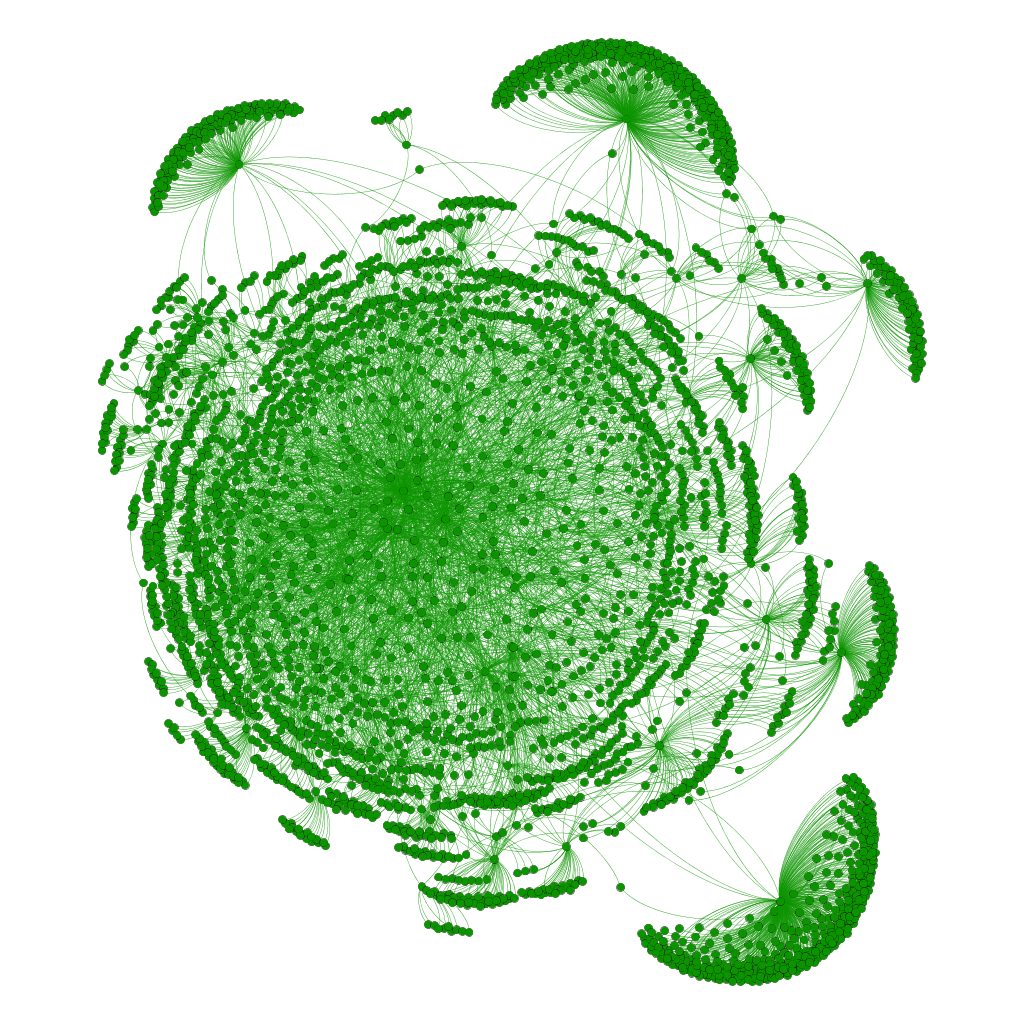
\includegraphics[width=0.5\textwidth]{GhostRATs.png}
    \caption{Graph of IP addresses, consisting of 3566 nodes with 204 known RAT controllers. The graph is visualized using Gephi.}
    \label{ip1}
\end{figure}

The second data set consists of 103202 NetFlow records collected during December 2016 to Mars 2017. This data set includes 10091 IP addresses but is far more sparse with \textit{Ghost}s, containing only 32 identified RAT controllers. 

The aim of this case is to classify IP addresses. This has been performed by applying similarity measures to the network. The applied similarity measures are the Dice coefficient, the Jaccard index, the cosine coefficient, the hub-promoting index and the hub-depressing index. This are all measures of structural equivalence and reflect the similarity based on the local structure. Noticeable is the fact that the similarity measures were calculated on an undirected graph due to the nature of the measures. 

The aim is partly to classify all the nodes given a small fraction of known nodes. Partly the aim is to identify false negatives, namely IP addresses that are falsely annotated as \textit{Non-ghost}s.

The similarity was calculated for all nodes, given a small portion (1-5) of known Gh0st RAT controllers, further refered to as reference nodes. Thus, the similarities for one node, in relation to the others, were simply taken as the sum. To classify the node, a threshold was then applied. 

Once the classification was performed, for different values of the threshold, the classifier based on different similarity measures was evaluated, based on the AUC of the precision recall curve and the F$_1$ score.

\subsection{Classification of malicious IP addresses}
- RF’s database
What IP addresses without a high risk score are likely to be malicious?
From Threat list: What IP addresses are added one week later? What similarities are there between the old and the new addresses? 

\subsection{Target and Attackers}
Which threat actors have similar profile? 
What entities are a part of another (bigger) entity?
Predict future attacks.


\newpage 
